\SourcePage{478}{481}
\chapter{Polyatomic molecules}
\setcounter{section}{99}
\setcounter{figure}{40}
\section{Classification of molecular vibrations}

For polyatomic molecules, the first task of group theory is to classify their electronic terms, that is, the energy levels belonging to a prescribed arrangement of the nuclei. The classification is by the irreducible representations of the point group possessed by the nuclear configuration under consideration. It must nevertheless be stressed that this classification applies to that particular arrangement of nuclei: displacing them will, in general, destroy the symmetry of the configuration. Usually the arrangement meant is the equilibrium one. The classification then retains a certain significance during small nuclear vibrations, but plainly ceases to do so when the vibrations can no longer be regarded as small.

This question did not arise for a diatomic molecule, since its axial symmetry is of course retained under every displacement of the nuclei. A similar circumstance holds for a triatomic molecule. Three nuclei always lie in one plane, and this is a symmetry plane of the molecule. Hence the electronic terms of a triatomic molecule can always be classified relative to that plane, according as the wave functions are symmetric or antisymmetric under reflection in it.

An empirical rule applies to the ground electronic terms of polyatomic molecules: for the great majority of molecules, the wave function of the ground electronic state is totally symmetric (this rule was already mentioned for diatomic molecules in \S~78). In other words, it is invariant under every element of the molecular symmetry group and therefore belongs to the identity irreducible representation of that group.

Group-theoretical methods are especially important in the investigation of molecular vibrations (E.~Wigner, 1930). Before treating this question quantum mechanically, one must first consider, entirely classically, the vibrations

\SourcePage{479}{482}
of a molecule regarded as a system of some number of interacting particles (the nuclei).

As is known from mechanics (see I, \S~23, 24), a system of $N$ particles not lying on one straight line has $3N-6$ vibrational degrees of freedom. Of the full set of $3N$ degrees of freedom, three describe translation and three describe rotation of the system as a whole\footnote{When all the particles lie on one straight line, there are $3N-5$ vibrational degrees of freedom. Only two coordinates then describe rotation, since rotation of a linear molecule about its own axis has no meaning.}. The energy of a particle system undergoing small vibrations can be written
\begin{equation}
 E=\frac12\sum_{i,k}m_{ik}\dot u_i\dot u_k+\frac12\sum_{i,k}k_{ik}u_i u_k. \tag{100.1}
\end{equation}
Here $m_{ik}$ and $k_{ik}$ are constant coefficients, while $u_i$ are components of the particle-displacement vectors measured from equilibrium (the indices $i,k$ label both vector components and particles). A suitable linear transformation of the $u_i$ eliminates from (100.1) the coordinates for translation and rotation of the system. The remaining vibrational coordinates can be chosen so that both quadratic forms in (100.1) become sums of squares. On normalizing these coordinates to make every coefficient in the kinetic energy equal to unity, the vibrational energy becomes
\begin{equation}
 E=\frac12\sum_{i,\alpha}\dot Q_{\alpha i}^{2}+\frac12\sum_\alpha\omega_\alpha^2\sum_i Q_{\alpha i}^{2}. \tag{100.2}
\end{equation}

The vibrational coordinates $Q_{\alpha i}$ are called \emph{normal coordinates}; the corresponding independent vibrations have frequencies $\omega_\alpha$. Several normal coordinates may have the same frequency, which is then called \emph{multiple}. In $Q_{\alpha i}$, the index $\alpha$ identifies the frequency, and $i=1,2,\ldots,f_\alpha$ enumerates the coordinates having that same frequency; $f_\alpha$ is its multiplicity.

Expression (100.2) for the energy of the molecule must be invariant under symmetry transformations. Thus, under each transformation in the molecule's point symmetry group, the normal coordinates $Q_{\alpha i}$, $i=1,2,\ldots,f_\alpha$, for any fixed $\alpha$, undergo linear transformations

\SourcePage{480}{483}
among themselves which leave the sum of squares $\sum_iQ_{\alpha i}^2$ unchanged. Put differently, the normal coordinates belonging to each natural frequency of the molecule furnish an irreducible representation of its symmetry group, and the frequency multiplicity is the dimension of that representation. Irreducibility follows from the same argument used in \S~96 for solutions of the Schrödinger equation. Equality of frequencies associated with two different irreducible representations would be an extraordinary accident. The earlier qualification must again be made: because physical normal coordinates are intrinsically real, two mutually conjugate complex representations correspond to a single natural frequency whose multiplicity is twice as large.

These observations allow the molecular normal modes to be classified without solving the difficult problem of finding their explicit normal coordinates. One first determines, by the procedure described below, the representation furnished jointly by all vibrational coordinates; call it the complete \emph{vibrational representation}. It is reducible. Resolving it into irreducible parts gives both the multiplicities of the natural frequencies and the symmetry properties of their modes. A given irreducible representation may occur several times in the complete representation. This signifies several distinct frequencies of the same multiplicity, with vibrations of identical symmetry.

To determine the complete vibrational representation, use the invariance of a representation's characters under a linear change of basis functions. Its characters may therefore be calculated by taking as basis functions not the normal coordinates but simply the components $u_i$ of the nuclear-displacement vectors from equilibrium.

To begin with, it is clear that, when finding the character of an element $G$ of the point group, one need consider only the nuclei left in place by the given symmetry transformation (more precisely, the nuclei whose equilibrium positions are left in place).

Indeed, suppose that under the rotation or reflection $G$, nucleus 1 moves to a new position previously occupied by another identical nucleus, nucleus 2. This means that the operation $G$ expresses the displacement of nucleus 1 in terms of the displacement of nucleus 2.

Thus, the rows of the matrix $G_{ik}$ associated with this nucleus (that is, with its displacement $u_i$) cannot, in any event, contain diagonal elements.

By contrast, the components of the displacement vector of a nucleus,

\SourcePage{481}{484}
whose equilibrium position is left unaffected by the operation $G$, are mapped one onto another only; they can therefore be treated separately from the displacement vectors of the remaining nuclei.

First consider a rotation $C(\varphi)$ through an angle $\varphi$ about a symmetry axis. Let $u_x,u_y,u_z$ be the components of the displacement vector of a nucleus whose equilibrium position lies on the axis and is consequently unchanged by the rotation. These components transform as those of an ordinary polar vector; with the $z$ axis chosen along the symmetry axis,
\[
 u_x'=u_x\cos\varphi+u_y\sin\varphi,\qquad
 u_y'=-u_x\sin\varphi+u_y\cos\varphi,\qquad
 u_z'=u_z.
\]
The character, namely the sum of the diagonal entries of the transformation matrix, is $1+2\cos\varphi$. If $N_C$ nuclei lie on the axis, their combined character is
\begin{equation}
 N_C(1+2\cos\varphi). \tag{100.3}
\end{equation}
This character, however, belongs to the transformation of all $3N$ displacements $u_i$. The parts describing translation and an infinitesimal rotation of the whole molecule must therefore be removed. Translation is specified by the centre-of-mass displacement vector $\mathbf U$, and its contribution to the character is consequently $1+2\cos\varphi$. Rotation of the entire molecule is described by the rotation-angle vector $\delta\boldsymbol\Omega$\footnote{An infinitesimal rotation angle can be regarded as a vector $\delta\boldsymbol\Omega$ whose magnitude is the angle and whose direction is along the rotation axis, with sense fixed by the screw rule. A vector defined in this manner is evidently axial.}.

Although $\delta\boldsymbol\Omega$ is axial, an axial vector transforms like a polar vector under rotations of the coordinate system. Its character is therefore also $1+2\cos\varphi$. Altogether, the quantity $2(1+2\cos\varphi)$ must be subtracted from (100.3). The character $\chi(C)$ of the rotation $C(\varphi)$ in the complete vibrational representation is thus
\begin{equation}
 \chi(C)=(N_C-2)(1+2\cos\varphi). \tag{100.4}
\end{equation}
For the identity element $E$, the character is simply the total number of vibrational degrees of freedom, $\chi(E)=3N-6$; this also follows from (100.4) by putting $N_C=N$ and $\varphi=0$.

\SourcePage{482}{485}
In the same way, consider the character of the rotation--reflection $S(\varphi)$, consisting of a rotation through $\varphi$ about the $z$ axis followed by reflection in the $xy$ plane. A vector then transforms according to
\[
 u_x'=u_x\cos\varphi+u_y\sin\varphi,\qquad
 u_y'=-u_x\sin\varphi+u_y\cos\varphi,\qquad
 u_z'=-u_z,
\]
whose character is $-1+2\cos\varphi$. Hence the representation furnished by all $3N$ displacements $u_i$ has character
\begin{equation}
 N_S(-1+2\cos\varphi), \tag{100.5}
\end{equation}
where $N_S$ is the number of nuclei left fixed by $S(\varphi)$; evidently this number can only be zero or one. The centre-of-mass displacement vector $\mathbf L$ contributes $-1+2\cos\varphi$. The vector $\delta\boldsymbol\Omega$, being axial, is invariant under inversion of the coordinate system. On the other hand, the rotation--reflection can be represented as
\[
 S(\varphi)=C(\varphi)\sigma_h=C(\varphi)C_2I=C(\pi+\varphi)I,
\]
that is, as a rotation through $\pi+\varphi$ followed by inversion. The character of $S(\varphi)$ acting on $\delta\boldsymbol\Omega$ is therefore the character of $C(\pi+\varphi)$ acting on an ordinary vector, namely $1+2\cos(\pi+\varphi)=1-2\cos\varphi$. Since $(-1+2\cos\varphi)+(1-2\cos\varphi)=0$, expression (100.5) itself is the required character $\chi(S)$ of $S(\varphi)$ in the complete vibrational representation:
\begin{equation}
 \chi(S)=N_S(-1+2\cos\varphi). \tag{100.6}
\end{equation}
In particular, reflection in a plane ($\varphi=0$) has character $\chi(\sigma)=N_\sigma$, while inversion ($\varphi=\pi$) has character $\chi(I)=-3N_I$.

Once the characters $\chi$ of the complete vibrational representation have been obtained, it remains only to decompose that representation into irreducible ones. Formula (94.16), together with the character tables in \S~95, performs this decomposition; see the problems to this section.

Group theory is unnecessary for classifying the vibrations of a linear molecule. The total number of vibrational degrees of freedom is $3N-5$. One must distinguish vibrations in which the atoms remain on one straight line from those

\SourcePage{483}{486}
in which they do not\footnote{If the molecule is symmetric about its midpoint, one further characteristic of the vibrations is available; see Problem 10 of this section.}. Motion of $N$ particles along a line has $N$ degrees of freedom, one of which describes translation of the whole molecule. Thus $N-1$ normal coordinates describe vibrations that keep the atoms collinear and correspond, in general, to $N-1$ distinct natural frequencies. The remaining $(3N-5)-(N-1)=2N-4$ normal coordinates describe bending vibrations. They correspond to $N-2$ distinct doubly degenerate frequencies, because each frequency has two normal coordinates for identical vibrations in two mutually perpendicular planes\footnote{In the notation for irreducible representations of $C_{\infty v}$ used in \S~98, there are $N-1$ vibrations of type $A_1$ and $N-2$ of type $E_1$.}.

\subsection*{Problems}

\ProblemHeading{1.} Classify the normal vibrations of the $\mathrm{NH_3}$ molecule (a regular pyramid with N at its apex and H atoms at the vertices of its base; Fig.~41).

\SolutionHeading The molecular point group is $C_{3v}$. Rotations about the threefold axis leave only one atom fixed (N), while each reflection plane fixes two atoms (N and one H). Equations (100.4) and (100.6) give the characters of the complete vibrational representation:
\[
\begin{array}{c|ccc} &E&2C_3&3\sigma_v\\\hline &6&0&2\end{array}
\]
\begin{figure}[ht]
\centering
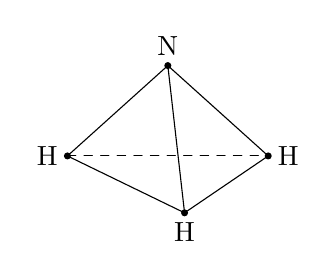
\begin{tikzpicture}[scale=.85,line cap=round]
\coordinate (N) at (0,1.35); \coordinate (L) at (-1.5,0); \coordinate (R) at (1.5,0); \coordinate (B) at (.25,-.85);
\draw (N)--(L)--(B)--(R)--cycle; \draw[dashed] (L)--(R); \draw (N)--(B);
\foreach \p in {N,L,R,B}\fill (\p) circle (1.5pt);
\node[above] at (N){N}; \node[left] at (L){H}; \node[right] at (R){H}; \node[below] at (B){H};
\end{tikzpicture}
\caption{}
\end{figure}
Decomposition into irreducible parts shows that the representation contains $A_1$ twice and $E$ twice. There are consequently two nondegenerate frequencies for modes of type $A_1$, which retain the full symmetry of the molecule (the so-called totally symmetric vibrations), and two doubly degenerate frequencies whose normal coordinates transform among themselves according to $E$.

\ProblemHeading{2.} Repeat the classification for $\mathrm{H_2O}$ (Fig.~42).

\begin{figure}[ht]
\centering
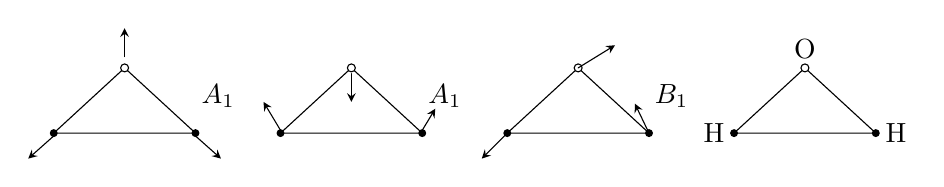
\begin{tikzpicture}[>=stealth,scale=.72,line cap=round]
\foreach \x/\lab in {0/$A_1$,4/$A_1$,8/$B_1$}{
 \coordinate (o) at (\x,1.15); \coordinate (l) at (\x-1.25,0); \coordinate (r) at (\x+1.25,0);
 \draw (l)--(o)--(r) (l)--(r); \fill (l) circle(2pt) (r) circle(2pt); \draw[fill=white] (o) circle(2pt); \node at (\x+1.65,.65){\lab};}
\draw[->] (0,1.35)--(0,1.85); \draw[->] (-1.25,-.05)--(-1.7,-.45); \draw[->] (1.25,-.05)--(1.7,-.45);
\draw[->] (4,1.05)--(4,.55); \draw[->] (2.75,.05)--(2.45,.55); \draw[->] (5.25,.05)--(5.48,.43);
\draw[->] (8,1.15)--(8.65,1.55); \draw[->] (6.75,0)--(6.3,-.45); \draw[->] (9.25,0)--(9.0,.52);
\coordinate (O) at (12,1.15); \coordinate (H1) at (10.75,0); \coordinate (H2) at (13.25,0); \draw (H1)--(O)--(H2) (H1)--(H2); \fill (H1) circle(2pt) (H2) circle(2pt); \draw[fill=white] (O) circle(2pt); \node[above] at (O){O}; \node[left] at (H1){H}; \node[right] at (H2){H};
\end{tikzpicture}
\caption{}
\end{figure}

\SolutionHeading The symmetry group is $C_{2v}$. The transformation $C_2$ fixes the O atom; $\sigma_v$, reflection in the molecular plane, fixes all three atoms; and $\sigma_v'$ fixes only O. The characters of the complete vibrational representation are
\[
\begin{array}{c|cccc}&E&C_2&\sigma_v&\sigma_v'\\\hline&3&1&3&1\end{array}
\]

\SourcePage{484}{487}
This representation decomposes as $2A_1+B_1$. Thus there are two totally symmetric vibrations and one whose symmetry is specified by $B_1$; every frequency is nondegenerate. The corresponding normal vibrations are drawn in Fig.~42.

\ProblemHeading{3.} Repeat for $\mathrm{CH_3Cl}$ (Fig.~43\textit{a}).

\SolutionHeading The molecular symmetry group is $C_{3v}$. The same procedure gives three totally symmetric $A_1$ vibrations and three doubly degenerate vibrations of type $E$.

\begin{figure}[p]
\centering
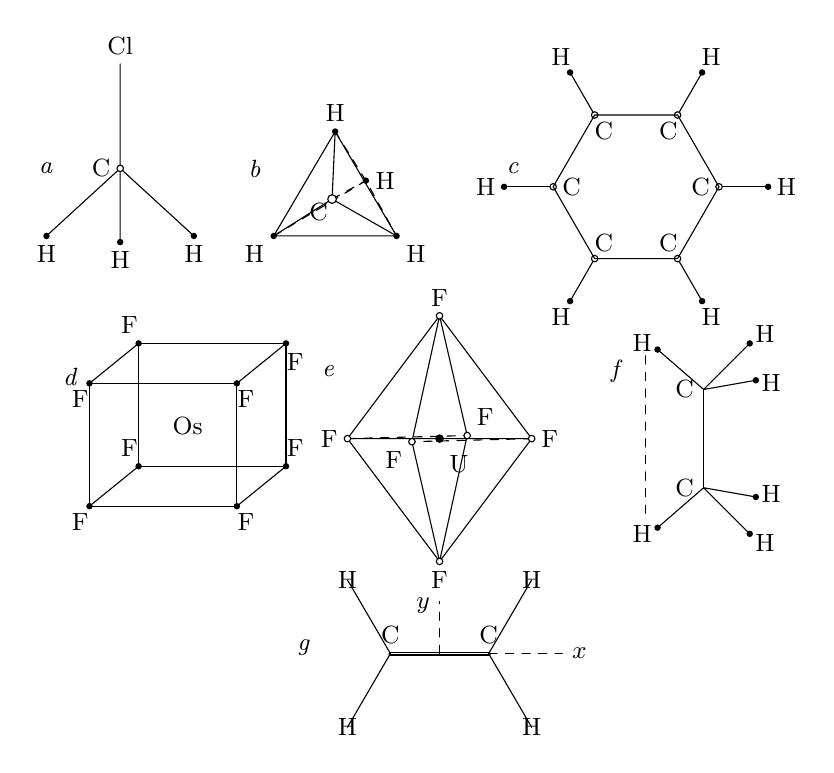
\begin{tikzpicture}[scale=.78,line cap=round,font=\small]
% a CH3Cl
\begin{scope}[shift={(-5.2,4.3)}]\node at (-1.2,.3){\textit{a}}; \coordinate(C)at(0,.3);\coordinate(Cl)at(0,2);\draw(C)--(Cl) (C)--(-1.2,-.8) (C)--(0,-.9) (C)--(1.2,-.8);\draw[fill=white](C)circle(1.5pt);\node[left]at(C){C};\node[above]at(Cl){Cl};\foreach\p in {(-1.2,-.8),(0,-.9),(1.2,-.8)}\fill\p circle(1.5pt);\node[below]at(-1.2,-.8){H};\node[below]at(0,-.9){H};\node[below]at(1.2,-.8){H};\end{scope}
% b CH4 tetrahedron
\begin{scope}[shift={(-1.7,4.3)}]\node at(-1.3,.3){\textit{b}};\coordinate(T)at(0,.9);\coordinate(L)at(-1,-.8);\coordinate(R)at(1,-.8);\coordinate(M)at(.5,.1);\coordinate(C)at(-.05,-.2);\draw(T)--(L)--(R)--cycle;\draw[dashed](L)--(M)--(R) (T)--(M);\draw(C)--(T) (C)--(L) (C)--(R);\draw[dashed](C)--(M);\draw[fill=white](C)circle(2pt);\fill(T)circle(1.5pt)(L)circle(1.5pt)(R)circle(1.5pt)(M)circle(1.5pt);\node[above]at(T){H};\node[below left]at(L){H};\node[below right]at(R){H};\node[right]at(M){H};\node[below left=-2pt]at(C){C};\end{scope}
% c benzene
\begin{scope}[shift={(3.2,4.3)}]\node at(-2,.3){\textit{c}};\foreach\i in{0,...,5}{\coordinate(C\i)at({60*\i}:1.35);\coordinate(H\i)at({60*\i}:2.15);\draw(C\i)--(H\i);\draw[fill=white](C\i)circle(1.5pt);\fill(H\i)circle(1.5pt);\node at({60*\i}:1.05){C};\node at({60*\i}:2.45){H};}\draw(C0)--(C1)--(C2)--(C3)--(C4)--(C5)--cycle;\end{scope}
% d cube OsF8
\begin{scope}[shift={(-4.5,.1)}]\node at(-1.5,1.1){\textit{d}};\draw(-1.2,-1)--(1.2,-1)--(1.2,1)--(-1.2,1)--cycle;\draw(-.4,-.35)--(2,-.35)--(2,1.65)--(-.4,1.65)--cycle;\draw(-1.2,-1)--(-.4,-.35) (1.2,-1)--(2,-.35) (1.2,1)--(2,1.65) (-1.2,1)--(-.4,1.65);\foreach\p in{(-1.2,-1),(1.2,-1),(1.2,1),(-1.2,1),(-.4,-.35),(2,-.35),(2,1.65),(-.4,1.65)}\fill\p circle(1.5pt);\node at(.4,.3){Os};\foreach\p in{(-1.35,-1.25),(1.35,-1.25),(1.35,.75),(-1.35,.75),(-.55,-.05),(2.15,-.05),(2.15,1.35),(-.55,1.95)}\node at\p{F};\end{scope}
% e UF6 octahedron
\begin{scope}[shift={(0,.2)}]\node at(-1.8,1.1){\textit{e}};\coordinate(T)at(0,2);\coordinate(B)at(0,-2);\coordinate(L)at(-1.5,0);\coordinate(R)at(1.5,0);\coordinate(F)at(-.45,-.05);\coordinate(K)at(.45,.05);\draw(T)--(L)--(B)--(R)--cycle (T)--(F)--(B) (T)--(K)--(B) (L)--(R);\draw[dashed](L)--(K) (R)--(F);\fill(0,0)circle(2pt);\node[below right]at(0,-.12){U};\foreach\p in{T,B,L,R,F,K}\draw[fill=white](\p)circle(1.5pt);\node[above]at(T){F};\node[below]at(B){F};\node[left]at(L){F};\node[right]at(R){F};\node[below left]at(F){F};\node[above right]at(K){F};\end{scope}
% f ethane
\begin{scope}[shift={(4.3,.2)}]\node at(-1.4,1.1){\textit{f}};\coordinate(Ct)at(0,.8);\coordinate(Cb)at(0,-.8);\draw(Ct)--(Cb);\node[left]at(Ct){C};\node[left]at(Cb){C};\foreach\p in{(-.75,1.45),(.75,1.55),(.85,.95),(-.75,-1.45),(.75,-1.55),(.85,-.95)}\fill\p circle(1.5pt);\draw(Ct)--(-.75,1.45) (Ct)--(.75,1.55) (Ct)--(.85,.95) (Cb)--(-.75,-1.45) (Cb)--(.75,-1.55) (Cb)--(.85,-.95);\foreach\p in{(-1,1.55),(1,1.7),(1.1,.9),(-1,-1.55),(1,-1.7),(1.1,-.9)}\node at\p{H};\draw[dashed](-.95,1.35)--(-.95,-1.35);\end{scope}
% g ethylene
\begin{scope}[shift={(0,-3.3)}]\node at(-2.2,.1){\textit{g}};\coordinate(CL)at(-.8,0);\coordinate(CR)at(.8,0);\draw[double](CL)--(CR);\node[above]at(CL){C};\node[above]at(CR){C};\draw(CL)--(-1.5,1.2) (CL)--(-1.5,-1.2) (CR)--(1.5,1.2) (CR)--(1.5,-1.2);\foreach\p in{(-1.5,1.2),(-1.5,-1.2),(1.5,1.2),(1.5,-1.2)}\node at\p{H};\draw[dashed](0,0)--(0,.85) (.8,0)--(2,0);\node[left]at(0,.78){$y$};\node[right]at(2,0){$x$};\end{scope}
\end{tikzpicture}
\caption{}
\end{figure}
\clearpage

\ProblemHeading{4.} Repeat for $\mathrm{CH_4}$, with C at the centre and H atoms at the vertices of a tetrahedron (Fig.~43\textit{b}).

\SolutionHeading The molecular symmetry is $T_d$. The vibrations are $1A_1$, $1E$, and $2F_2$.

\ProblemHeading{5.} Repeat for $\mathrm{C_6H_6}$ (Fig.~43\textit{c}).

\SolutionHeading The molecular symmetry is $D_{6h}$. The vibrations are
\[
2A_{1g},1A_{2g},1A_{2u},1B_{1g},1B_{1u},1B_{2g},3B_{2u},1E_{1g},3E_{1u},4E_{2g},2E_{2u}.
\]

\ProblemHeading{6.} Repeat for $\mathrm{OsF_8}$, with Os at the centre and F atoms at the cube vertices (Fig.~43\textit{d}).

\SolutionHeading The molecular symmetry is $O_h$. The vibrations are
\[
1A_{1g},1A_{2u},1E_g,1E_u,2F_{1u},2F_{2g},2F_{2u}.
\]

\ProblemHeading{7.} Repeat for $\mathrm{UF_6}$, with U at the centre and F atoms at the octahedron vertices (Fig.~43\textit{e}).

\SourcePage{485}{488}
\SolutionHeading The molecular symmetry is $O_h$. The vibrations are
\[
1A_{1g},1E_g,2F_{1u},1F_{2g},1F_{2u}.
\]

\ProblemHeading{8.} Repeat for $\mathrm{C_2H_6}$ (Fig.~43\textit{f}).

\SolutionHeading The molecular symmetry is $D_{3d}$. The vibrations are
\[
3A_{1g},1A_{1u},2A_{2u},3E_g,3E_u.
\]

\ProblemHeading{9.} Repeat for $\mathrm{C_2H_4}$; all its atoms are coplanar (Fig.~43\textit{g}).

\SolutionHeading The molecular symmetry is $D_{2h}$. The vibrations are
\[
3A_{1g},1A_{1u},2B_{1g},1B_{1u},2B_{3u},1B_{2g},2B_{2u}
\]
(the coordinate axes are chosen as shown in the figure).

\ProblemHeading{10.} Repeat for a linear molecule of $N$ atoms which is symmetric about its midpoint.

\SolutionHeading The classification already given for the vibrations of a linear molecule must be supplemented by their behaviour under inversion in the centre. The cases of even and odd $N$ must be treated separately.

Let $N$ be even, $N=2p$, so that there is no atom at the molecular midpoint. Assign independent displacements along the line to the $p$ atoms in one half of the molecule, and equal opposite displacements to the other $p$ atoms. This shows that $p$ of the modes preserving collinearity are symmetric about the centre; the remaining $(2p-1)-p=p-1$ modes of this kind are antisymmetric. Next, the $p$ atoms have $2p$ degrees of freedom for motions that do not constrain them to the line. Equal opposite displacements of symmetrically situated atoms would give $2p$ symmetric modes, but two modes describing molecular rotation must be subtracted. There are therefore $p-1$ doubly degenerate bending frequencies symmetric about the centre, and the same number, $(2p-2)-(p-1)=p-1$, which are antisymmetric. In the notation of irreducible representations of $D_{\infty h}$ used at the end of \S~98, there are $p$ vibrations of type $A_{1g}$ and $p-1$ vibrations of each of the types $A_{1u}$, $E_{1g}$, and $E_{1u}$.

If $N$ is odd, $N=2p+1$, the same reasoning gives $p$ vibrations of each of the types $A_{1g}$, $A_{1u}$, and $E_{1u}$, together with $p-1$ of type $E_{1g}$.
